\documentclass[9pt]{beamer}

\usetheme[progressbar=frametitle]{metropolis}
\usepackage{appendixnumberbeamer}
\usepackage[alf, bibjustif]{abntex2cite}
\usepackage{booktabs}
\usepackage[scale=2]{ccicons}
\usepackage{pgfplots}
\usepgfplotslibrary{dateplot}
\usepackage[utf8]{inputenc}
\usepackage[T1]{fontenc}
\usepackage[brazil]{babel}
\usepackage{xspace}
\usepackage{graphicx}
\usepackage{mathtools}
\usepackage{bclogo}

\newcommand{\themename}{\textbf{\textsc{metropolis}}\xspace}


\begin{document}

\title{Do lulismo ao antipetismo?}
\subtitle{Polarização, partidarismo e voto nas eleições presidenciais brasileiras}
\author{André Borges e Robert Vidigal}
\date{}
\institute{\textit{Opinião Pública}, Campinas, vol. 24, n. 1, jan.-abr., 2018}

\maketitle

\begin{frame}{Estado da Arte}
    \begin{itemize}
        \item A disputa presidencial no contexto de embate entre PT e PSDB estrutura o sistema partidário; 
        \item Identificação partidária é fator significativo para a decisão do voto em eleições presidenciais;
        \item \textbf{Pergunta}: como medir identificação partidária?
    \end{itemize}
\end{frame}

\begin{frame}{Questões}
    \begin{enumerate}
        \item Os eleitores se dividem em polos na disputa presidencial ao longo do tempo? Se sim, em que grau essa polarização ocorre?
        \item Houve polarização partidária na competição PT $\times$ PSDB?
        \item Qual foi o impacto das \textit{simpatias partidárias} sobre o voto presidencial entre 2002 e 2014?
    \end{enumerate}

\textbf{Objeto:} \textit{surveys} do Estudo Eleitoral Brasileiro (Eseb) realizados entre 2002 e 2014, desenvolvendo uma escala de \textit{partidarismo}.
\end{frame}

\begin{frame}{Uma medida de polarização}
Considera que nenhuma das teorias clássicas explica a identificação partidária nas novas democracias. 
   \begin{description}
       \item[Teoria de grupos:] medir polarização considerando os sentimentos negativos e positivos dos eleitores pelos partidos "polarizadores".
   \end{description}

    Não se trata de analisar a identificação partidária negativa, mas a \textbf{polarização de massa} \cite[~p. 55]{borges}

    \begin{description}
        \item[Ajuste comparativo:] "[...] os indivíduos se classificam em grupos não apenas quando eles acham que se assemelham, ou se ajustam, àquele grupo, mas também quando eles acreditam que seu grupo difere dos outros (Lupu, 2013)." \cite[~p. 57]{borges}
    \end{description}
\end{frame}


\begin{frame}{O que é polarização?}
    \begin{figure}[h]
        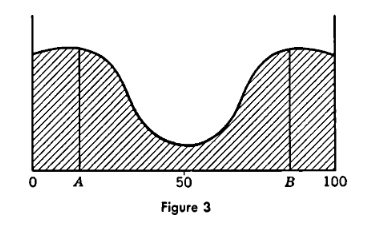
\includegraphics[width=9cm]{images/Downs.png}
        \caption{Distribuição polarizada do eleitorado \cite[~p. 119]{downs}}
    \end{figure}
\end{frame}

\begin{frame}{Limites da identificação partidária}
    \begin{itemize}
        \item Escolarização;
        \item Fragmentação e falta de nitidez do sistema partidário.
    \end{itemize}

    Mesmo assim, a literatura converge no argumento de que a eleição presidencial ancora o sistema. Mais do que isso:

    \begin{itemize}
        \item Há um processo de fortalecimentos dos sentimentos em relação aos partidos;
        \item Aprofundamento da polarização (reação às políticas redistributivas do PT --- clivagens sociais).
    \end{itemize}
\end{frame}

\begin{frame}{Hipóteses}
Dada a literatura, podemos esperar:
    \begin{description}
        \item[H1:] ao longo do tempo, aumento na intensidade dos sentimentos partidários (positivos e negativos) em relação aos dois partidos presidenciais;
        \item[H2:] maior grau de diferenciação de atitudes dos eleitores que simpatizam com um ou outro partido (polarização);
        \item[H3:] deve ter havido uma queda na probabilidade de voto em terceiros candidatos entre aqueles que simpatizam com PT ou PSDB em relação aos eleitores não identificados (complementarmente, aumento da capacidade explicativa das simpatias partidárias em detrimento da capacidade explicativa de dimensões de curto prazo).
    \end{description}
\end{frame}

\begin{frame}{Metodologia --- \textit{classificando o eleitor}}
    \begin{figure}[h]
        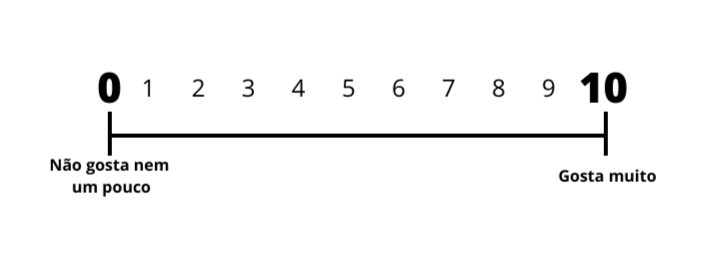
\includegraphics[width=9cm]{images/escala.png}
        \caption{Pergunta do Eseb}
    \end{figure}

\end{frame}

\begin{frame}{Metodologia --- \textit{classificando o eleitor}}
Se $x = (scorePT, scorePSDB)$, daí:
$$f(x) = scorePT - scorePSDB$$

E, então:
$$g(f(x)) = \begin{cases}
    \text{puro, se } |f(x)| > 6, \\
    \text{moderado, se } 4 \leq |f(x)| \leq 6, \\ 
    \text{indiferente, caso contrário.}
\end{cases}$$

Finalmente, $$h(g(f(x))) = \begin{cases}
    +2, \text{se petista puro}, \\
    -2, \text{se tucano puro}, \\
    +1, \text{se petista moderado}, \\
    -1, \text{se tucano moderado}, \\
    0, \text{se indiferente}.
\end{cases}$$
\end{frame}

\begin{frame}{Distribuição da identificação partidária --- Teste da H1}
    \begin{figure}[h]
        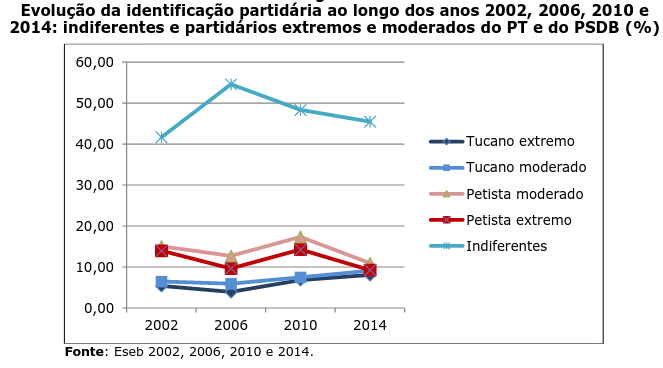
\includegraphics[width=10cm]{images/eleitores.png}
        \caption{Distribuição da identificação partidária do eleitorado ao longo do tempo.}
    \end{figure}
\end{frame}

\begin{frame}{Antipetistas independentes --- Teste da H1}
    \begin{figure}[h]
        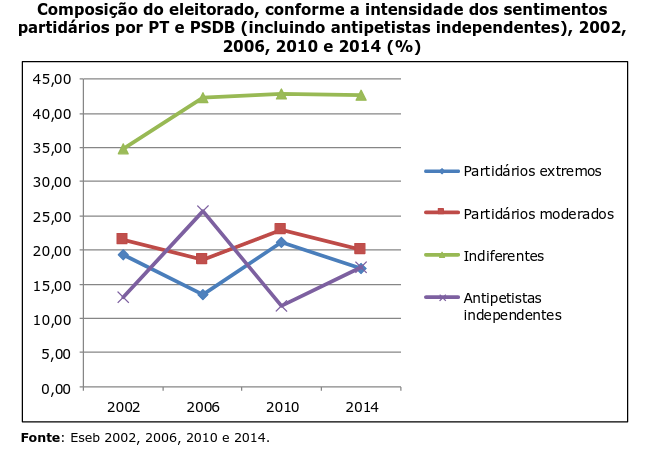
\includegraphics[width=9cm]{images/antipetistas.png}
        \caption{Antipetistas independentes.}
    \end{figure}
\end{frame}

\begin{frame}{Teste da H2}
    \begin{figure}[ht]
        \begin{minipage}[b]{0.6\linewidth}
            \centering
            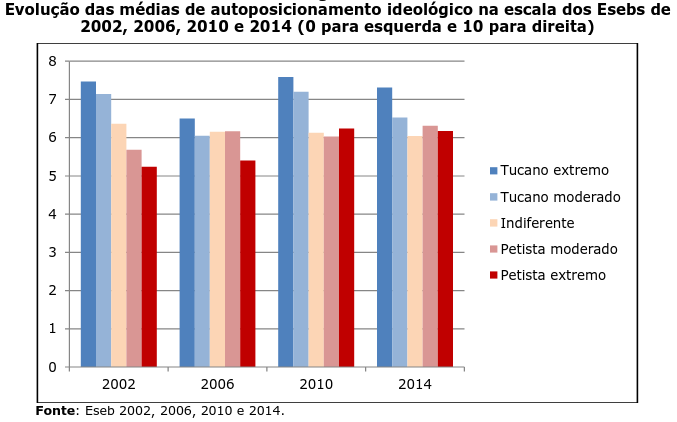
\includegraphics[width=7.5cm]{images/medias.png}
            \label{fig:a}
        \end{minipage}
        \hspace{0.8cm}
        \begin{minipage}[b]{0.6\linewidth}
            \centering
            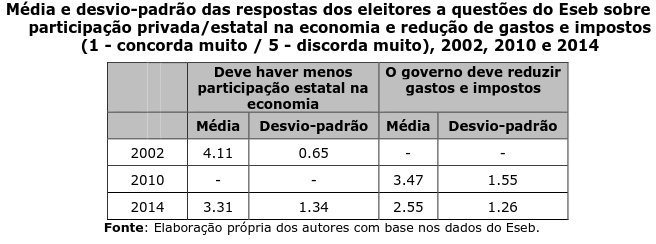
\includegraphics[width=7.5cm]{images/tabela.png}
            \label{fig:b}
        \end{minipage}
    \end{figure}
\end{frame}

\begin{frame}{Teste de médias --- Teste da H2}
    \begin{figure}[h]
        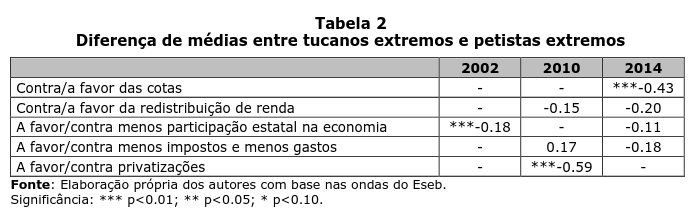
\includegraphics[width=9cm]{images/teste de medias.png}
        \caption{Antipetistas independentes.}
    \end{figure}
\end{frame}

\begin{frame}{Posicionamento ideológico médio --- Teste da H2}
    \begin{figure}[h]
        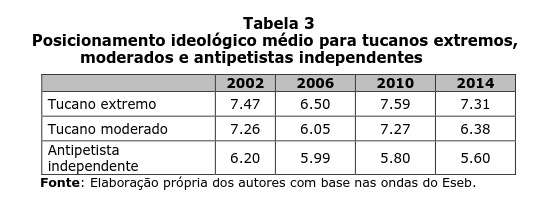
\includegraphics[width=8cm]{images/posicionamento ideologico medio.png}
    \end{figure}
\end{frame}

\begin{frame}{Modelos multivariados}

Antes, algumas considerações:

\begin{description}
    \item[Regressão linear:] queremos, considerando dados previamente observados, estimar qual o número aproximado de votos que um candidato deve obter em determinada eleição.

    \textit{Output:} um número.
    
    \item[Regressão logística:] queremos, considerando dados previamente observados, prever se um candidato será ou não reeleito em determinada eleição.

    \textit{Output:} uma classificação.
\end{description}

Um modelo de regressão multinomial (utilizado no artigo) é semelhante à logística, na medida em que escolhemos uma variável de referência e estimamos os coeficientes de uma combinação linear no processo de regressão \cite{kellstedt_whitten}. No entanto, a variável dependente não está restrita a duas categorias.

\end{frame}

\begin{frame}{Estimação dos determinantes do voto no primeiro turno}

Variável dependente:

\begin{itemize}
    \item Voto em candidatos não filiados ao PT ou PSDB (categoria-base);
    \item Voto branco/nulo (1);
    \item Voto no PSDB (2);
    \item Voto no PT (3).
\end{itemize}

As principais variáveis independentes são as medidas de simpatia partidária: $$\begin{cases}
    0, \text{se indiferente,} \\
    -1, \text{se tucano moderado/extremo,} \\
    +1, \text{se petista moderado/extremo}
\end{cases}$$

\end{frame}

\begin{frame}{Estimação dos determinantes do voto no primeiro turno}
    \begin{figure}[h]
        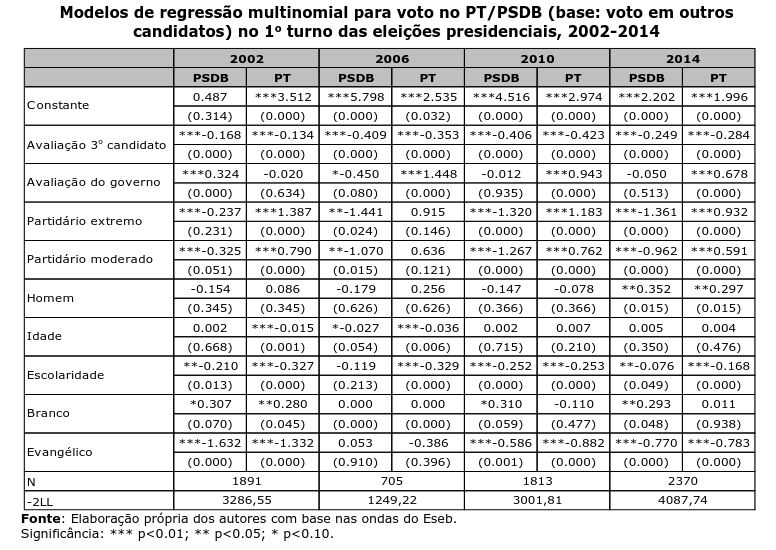
\includegraphics[width=9cm]{images/regressao1.png}
    \end{figure}
\end{frame}

\begin{frame}{Teste da H3}
    Testagem a partir de dois modelos: um incluindo apenas variáveis de simpatia partidária e outro incluindo apenas medidas de avaliação (\textit{teste de razão de verossimilhança e estatística -2LL}).
    \begin{figure}[h]
        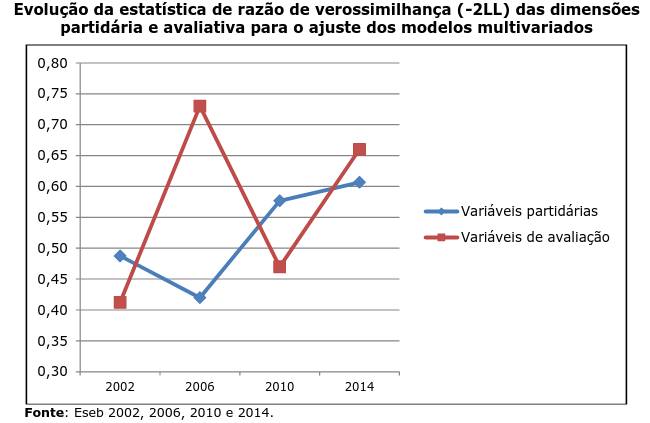
\includegraphics[width=8cm]{images/2ll.png}
    \end{figure}
\end{frame}

\begin{frame}{Nem petista, nem tucano}
    \begin{figure}[h]
        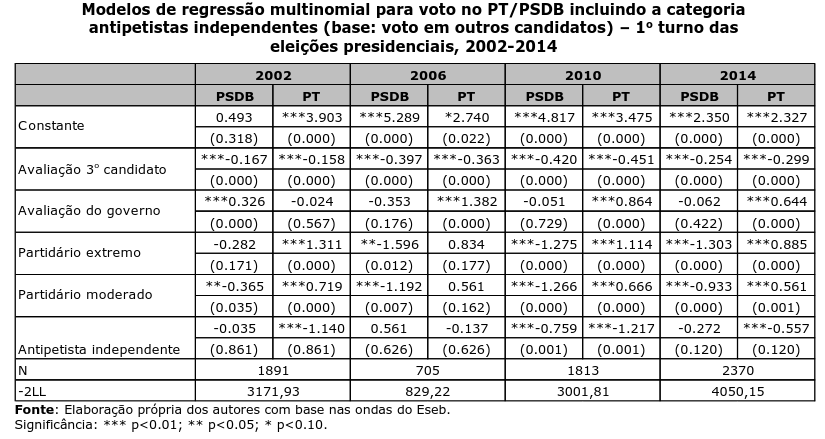
\includegraphics[width=9cm]{images/voto antipetista.png}
    \end{figure}
\end{frame}

\begin{frame}{Média de probabilidades --- Teste da H3}
    \begin{figure}[h]
        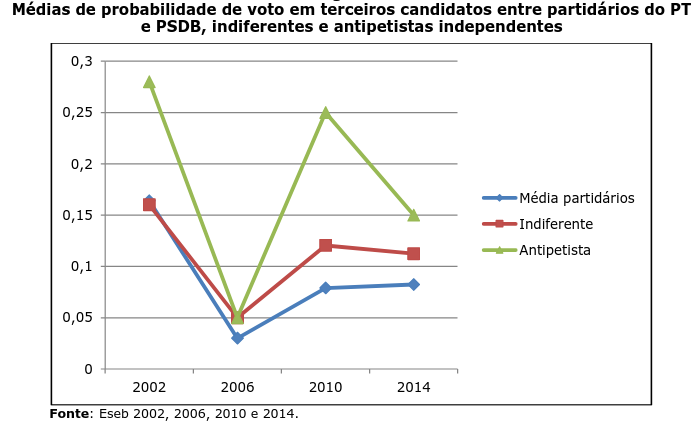
\includegraphics[width=8cm]{images/media de probabilidade.png}
    \end{figure}
\end{frame}

\begin{frame}{Conclusões}
    \begin{enumerate}
        \item Hipóteses que indicam crescimento da polarização partidária são empiricamente frágeis, "[...] especialmente no que diz respeito a um suposto crescimento da direita entre o eleitorado." \cite[p. ~78]{borges};
        \item O eleitorado convergiu ideologicamente ao longo do tempo e o eleitorado petista não possui perfil ideológico claro. Antipetistas se diferenciam menos dos petistas do que os eleitores tucanos;
        \item Parte expressiva dos eleitores não está disposta a apoiar ativamente qualquer um dos dois partidos;
        \item Antipetistas independentes procuram candidatos alternativos ao PT no primeiro turno, mas também não busca o candidato do PSDB.
    \end{enumerate}

E, por fim... \bcsmmh

\end{frame}

\begin{frame}{Aspa forte}
    Os céticos poderão argumentar que nossa análise não permite entender o fenômeno Bolsonaro, candidato de extrema-direita que aparece agora (dezembro de 2017) com cerca de 15\% nas pesquisas de intenção de voto para presidente em 2018. Sobre isso, cabe notar que pesquisas realizadas com tanta antecedência têm capacidade preditiva limitada. [...]

    [...]

    [...] Em resumo, em combinação com o sistema de dois turnos, que induz fortemente os partidos a mobilizar o eleitor mediano, desfavorecendo candidaturas extremistas, a distribuição das preferências do eleitorado brasileiro torna improvável um cenário de aumento da polarização partidária nos próximos anos, não obstante os diagnósticos (equivocados) a respeito do crescimento do eleitorado de extrema-direita no Brasil. \cite[p. ~80]{borges}
\end{frame}

\begin{frame}{Referências bibliográficas}
\bibliography{references}
\nocite{}
\end{frame}

\begin{frame}{}
$$\text{Prediction is very difficult, especially if it's about the future!}$$
$$\text{- Niels Bohr}$$
\end{frame}

\end{document}
